\documentclass[11pt,a4paper]{article}
\usepackage{amsmath,amsthm,amsfonts,amssymb,amscd}
\usepackage{enumerate} 
\usepackage{physics}
\usepackage{enumerate}
\usepackage{fancyhdr}
 \usepackage{hyperref}
\hypersetup{colorlinks,
    linkcolor=blue,
    citecolor=blue,      
    urlcolor=blue,
}
\usepackage{graphicx}


\oddsidemargin0.1cm 
\evensidemargin0.8cm
\textheight22.7cm 
\textwidth15cm \topmargin-0.5cm

\newtheorem{theorem}{Theorem}[section]
\newtheorem{lemma}[theorem]{Lemma}

\usepackage{listings}
\usepackage{xcolor}

\definecolor{codegreen}{rgb}{0,0.6,0}
\definecolor{codegray}{rgb}{0.5,0.5,0.5}
\definecolor{codepurple}{rgb}{0.58,0,0.82}
\definecolor{backcolour}{rgb}{0.95,0.95,0.92}

\lstdefinestyle{mystyle}{
    backgroundcolor=\color{backcolour},   
    commentstyle=\color{codegreen},
    keywordstyle=\color{magenta},
    numberstyle=\tiny\color{codegray},
    stringstyle=\color{codepurple},
    basicstyle=\ttfamily\footnotesize,
    breakatwhitespace=false,         
    breaklines=true,                 
    captionpos=b,                    
    keepspaces=true,                 
    numbers=left,                    
    numbersep=5pt,                  
    showspaces=false,                
    showstringspaces=false,
    showtabs=false,                  
    tabsize=2
}

\lstset{style=mystyle}

\newcommand{\silvia}[1]{{ {\color{blue}{(silvia)~#1}}}}
\newcommand{\grace}[1]{{ {\color{purple}{(grace)~#1}}}}

\newcommand{\MultiSet}{\mathrm{MultiSet}}
\newcommand{\len}{\mathrm{len}}
\newcommand{\din}{\texttt{d\_in}}
\newcommand{\dout}{\texttt{d\_out}}
\newcommand{\T}{\texttt{T} }
\newcommand{\F}{\texttt{F} }
\newcommand{\Relation}{\texttt{Relation}}
\newcommand{\X}{\mathcal{X}}
\newcommand{\Y}{\mathcal{Y}}
\newcommand{\True}{\texttt{True}}
\newcommand{\False}{\texttt{False}}
\newcommand{\clamp}{\texttt{clamp}}
\newcommand{\function}{\texttt{function}}
\newcommand{\float}{\texttt{float }}
\newcommand{\questionc}[1]{\textcolor{red}{\textbf{Question:} #1}}

\title{Privacy Proofs for OpenDP: Row Transform}
\author{Grace Tian}
\date{Summer 2021}
\begin{document}

\maketitle
\tableofcontents


\section{Algorithm Implementation}
\subsection{Code in Rust}
The current OpenDP library contains the \texttt{make\_row\_by\_row} function implementing the row transform function. This is defined in lines 10-26 of the file \texttt{manipulation.rs} in the Git repository (\url{https://github.com/opendp/opendp/blob/main/rust/opendp/src/trans/manipulation.rs#L10-L26}).

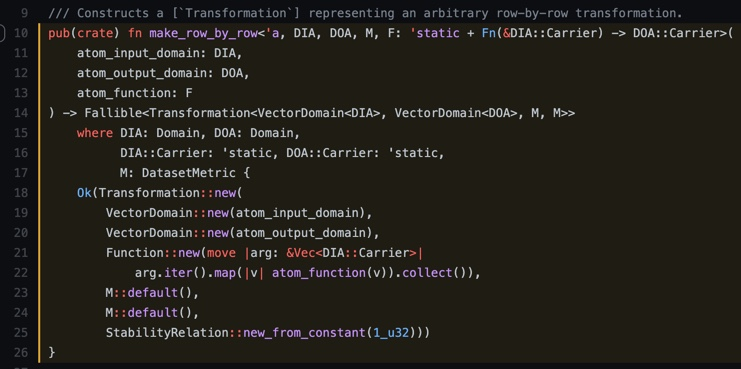
\includegraphics[width=\textwidth]{make_row_by_row.jpg}


\subsection{Pseudo Code in Python} \label{sec:pseudocode}

\subsection*{Preconditions}
To ensure the correctness of the output, we require the following preconditions:

\begin{itemize}
    \item \textbf{User-specified types:}
    \begin{itemize}
        \item Variable \texttt{atom\_input\_domain} has type \texttt{DIA}
        \item Variable \texttt{atom\_output\_domain} has type \texttt{DOA}
        \item Variable \texttt{atom\_function} has type \texttt{F}
        \item Types \texttt{DIA} and \texttt{DOA} have trait \texttt{Domain}
        \item Type \texttt{F} has trait \texttt{Fn(\&DIA::Carrier) -> DOA::Carrier)} 
    \end{itemize}
\end{itemize}

\subsection*{Postconditions}
\begin{itemize}
    \item Either a valid \texttt{Transformation} is returned or an error is returned.
\end{itemize}


\begin{lstlisting}[language=Python, escapechar=|]
def make_row_by_row(atom_input_domain : DIA, atom_output_domain : DOA, atom_function : F):
    input_domain = VectorDomain(DIA);
    output_domain = VectorDomain(DOA)
    input_metric = SymmetricDistance()
    output_metric = SymmetricDistance()

    def Relation(d_in : u32, d_out : u32) -> bool: |\label{line:rel}|
        return d_out <= d_in*1
    
    def function(data : Vec[DIA]) -> Vec[DOA]:  |\label{line:fn}|
        return list(map(atom_function, data)) |\label{line:map}|
    
    return Transformation(input_domain, output_domain, function, input_metric, output_metric, stability_relation=Relation)

\end{lstlisting}


\section{Proof}
The necessary definitions for the proof can be found at \href{https://www.overleaf.com/project/60d214e390b337703d200982}{``List of definitions used in the proofs"}.

\begin{theorem}
    For every setting of the input parameters \texttt{(atom\_input\_domain, atom\_output\_domain, atom\_function)} to \texttt{make\_row\_by\_row} such that the given preconditions
    hold, the transformation returned by \texttt{make\_row\_by\_row} has the following properties:
    \begin{enumerate}
        \item \textup{(Appropriate output domain).} For every element $v$ in \texttt{input\_domain}, $\function(v)$ is in \texttt{output\_domain}. 
        
        \item \textup{(Domain-metric compatibility).} The domain \texttt{input\_domain} matches one of the possible domains listed in the definition of \texttt{input\_metric}, and likewise \texttt{output\_domain} matches one of the possible domains listed in the definition of \texttt{output\_metric}.
        
        \item \textup{(Stability guarantee).} For every pair of elements $v, w$ in \texttt{input\_domain} and for every pair $(\din, \dout)$, where $\din$ is of the associated type for \texttt{input\_metric} and $\dout$ is the associated type for \texttt{output\_metric}, if $v,w$ are $\din$-close under \texttt{input\_metric} and $\Relation(\din, \dout) = \True$, then $\function(v), \function(w)$ are $\dout$-close under \texttt{output\_metric}.
    \end{enumerate}
\end{theorem}
\begin{proof}
\begin{enumerate}
\item \textbf{(Appropriate output domain).} In the case of \texttt{make\_row\_by\_row}, this corresponds to showing that for every vector $v$ of elements of type \texttt{DIA}, \texttt{function}$(v)$ is a vector of elements of type \texttt{DOA}. 

The $\function(v)$ has type \texttt{Vec[DOA]} follows from the assumption that element $v$ is in \texttt{input\_domain} and from the type signature of \texttt{function} in line~\ref{line:fn} of the pseudocode (Section~\ref{sec:pseudocode}), which takes in an element of type \texttt{Vec(DIA)} and returns an element of type \texttt{Vec[DOA]}. If the Rust code compiles correctly, then the type correctness follows from the definition of the type signature enforced by Rust. Otherwise, the code raises a compile time error for incorrect input type. \grace{Silvia wrote that it raises compile time error for incorrect input type, does it do the same for incorrect output type?}


\grace{I think checking type signature is sufficient for this pf.}

\item \textbf{(Domain-metric compatibility).} The Symmetric distance is both the \texttt{input\_metric} and \texttt{output\_metric}. Symmetric distance is compatible with \texttt{VectorDomain(T)} for any generic type \texttt{T}, as stated in \href{https://www.overleaf.com/project/60d215bf90b337ac02200a99}{``List of definitions used in the pseudocode"}. The theorem holds because for \texttt{make\_row\_by\_row}, the input domain is \texttt{VectorDomain(DIA)} and the output domain is \texttt{VectorDomain(DOA)}. 


\item \textbf{(Stability guarantee).} From Lemma 3.1 in \href{https://www.overleaf.com/project/60d214e390b337703d200982}{``List of definitions used in the proofs"} on the symmetric distance of row transform, we know that $$d_{Sym}(\texttt{function}(v), \texttt{function}(w)) \leq d_{Sym}(v, w).$$

Because $\Relation(\din, \dout) = \texttt{True}$, it follows that $\din \leq \dout$ by the \texttt{is\_equal} stability relation defined in the pseduocode. Since vector inputs $v, w$ are $\din$-close, then the symmetric distance is bounded by $\din$ by definition the symmetric distance is bounded by $d_{in}$: $d_{Sym}(v, w) \leq \din$. It finally follows that the transformations are \dout-close: $d_{Sym}(\function(v), \function(w)) \leq \dout$.
\end{enumerate}
\end{proof}

\end{document}

